\documentclass[runningheads,a4paper]{llncs}
\usepackage[utf8]{inputenc}
\usepackage[hyphens]{url}
\usepackage{graphicx}
\usepackage{hyperref}
\usepackage{float}
\usepackage{eurosym}
\usepackage[normalem]{ulem}
\usepackage{alltt}
\usepackage{subfig}
\usepackage{amssymb}
\setcounter{tocdepth}{3}

\usepackage{url}
\newcommand{\keywords}[1]{\par\addvspace\baselineskip
\noindent\keywordname\enspace\ignorespaces#1}

\begin{document}

\mainmatter  % start of an individual contribution

% first the title is needed
\title{Context-aware Querying for\\ Multi-modal Search Engines}

% a short form should be given in case it is too long for the running head
\titlerunning{Context-aware Querying for Multi-modal Search Engines}

\author{Jonas Etzold\inst{1}, Arnaud Brousseau\inst{2} Paul Grimm\inst{1} and Thomas Steiner\inst{2}}

\authorrunning{Context-aware Querying for Multi-modal Search Engines}
% (feature abused for this document to repeat the title also on left hand pages)

% the affiliations are given next; don't give your e-mail address
% unless you accept that it will be published
\institute{Erfurt University of Applied Sciences, Germany, \email{\{jonas.etzold|grimm\}@fh-erfurt.de}
\and Google Germany GmbH, ABC-Str. 19, 20354 Hamburg, Germany, \email{\{arnaudb|tomac\}@google.com}}

\maketitle

\begin{abstract}
(Tom)
\keywords{lorem, ipsum}
\end{abstract}

\section{Introduction}
(Tom) \cite{ijmis}

\section{Related Work}
(Jonas) \cite{nigay}

\section{Methodology}
(Arnaud, Jonas)

\subsection{MMBag}

MMBag stands for Multi-Media Bag and designates the I-SEARCH User Interface. It comes with specific requirements linked with the need for users to use multiple types of input: audio files or stream, video files, 3D objects, hand drawings, real-world information such as geolocation or time, image files and of course, plain text. This part of the paper tries to show the approach chosen to create MMBag.

Multi-modal search engines are still very experimental at the time of writing. When building MMBag, we tried to look for a common pattern in search-related actions. Indeed, MMBag remains a search interface at its core. In order for users to interact efficiently with I-SEARCH, we needed a well-known interface paradigm. Accross the web, a pattern has the monopoly for search related actions:  the text field, where a user can focus, enter his/her query, and trigger subsequent search action. From big search corporations such as Google, Yahoo or Bing, to small internal searches, the pattern stays the same. 

However, I-SEARCH can't directly benefit from this broadly accepted pattern. Indeed, a multi-modal search engine must accept a large number of types of input at the same time: audio, video, 3D objects, sketches, etc. How can this be achieved?
 
Some search engines, even if they don't have the need for true multi-modal querying, do have the need to accept input which is not plain text.

A first example of that is TinEye\footnote{\url{http://www.tineye.com/}}. TinEye is a web-based search engine which enables queries by picture, in order to retrieve similar or related images. 
\begin{figure}[h!]
  \centering
    
\includegraphics[width=0.8\linewidth]{resources/tineye-UI.png}
  \caption{Extract from the TinEye User Interface}
  \label{fig:tineye-ui}
\end{figure}

The interface is split in two distincts parts: one part is a text box to provide a link of a web hosted picture while the second part allow for direct file upload. This interface is a good solution for a search engine like TinEye (image input, image output) but I-SEARCH will need to come with more options than that.

 For example, let's have a look at MMRetrieval. It is an attempt at bringing together image and text search, i.e., combining pictures and plain text to compose a multi-modal query. MMRetrieval shows how cluttered an interface can become as more options are given to the user. To many, unclear  options are featured on the interface, making the process of query formulation long and difficult.

\begin{figure}[h!]
  \centering
    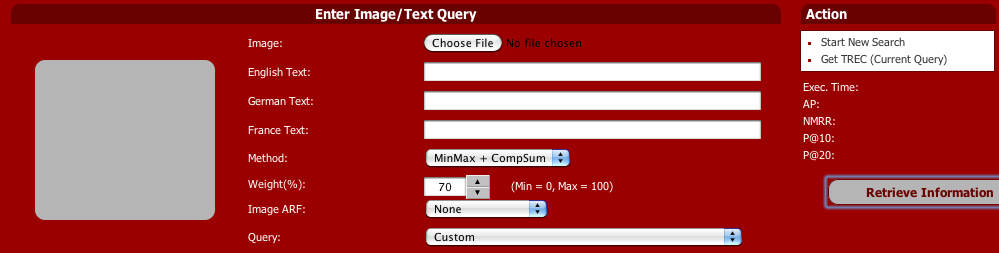
\includegraphics[width=0.8\linewidth]{resources/mmretrieval-UI.png}
  \caption{Extract from the MMRetrieval User Interface}
  \label{fig:mmretrieval-ui}
\end{figure}

Finally, we can have a look at Google Search-by-image. This functionnality was lauched on June, 14th 2011\footnote{\url{http://googleblog.blogspot.com/2011/06/knocking-down-barriers-to-knowledge.html}} and has the same requirements as MMRetrieval in terms of user interface, i.e., combining text and image input. 

\begin{figure}[h!]
  \centering
    
\includegraphics[width=0.8\linewidth]{resources/search-by-image-UI-box.png}
  \caption{Input for the Search-by-image UI}
  \label{fig:search-by-image-box}
\end{figure}

\begin{figure}[h!]
  \centering
    
\includegraphics[width=0.8\linewidth]{resources/search-by-image-UI-popup.png}
  \caption{Popup for the Search-by-image UI}
  \label{fig:search-by-image-popup}
\end{figure}

With the Search-by-image interface, Google has succeeded in keeping the text box pattern, while preventing any extra visual noise. The interface is \emph{progressively disclosed} to users via a contextual menu when the camera icon is clicked.

Even if the Search-by-image solution seems very elegant, this is still not suitable for I-SEARCH since the interface would require a high number of small icons: camera, 3d, geolocation, audio, video, etc.  As a result, we decided to adapt this solution. 

\begin{figure}[h!]
  \centering
    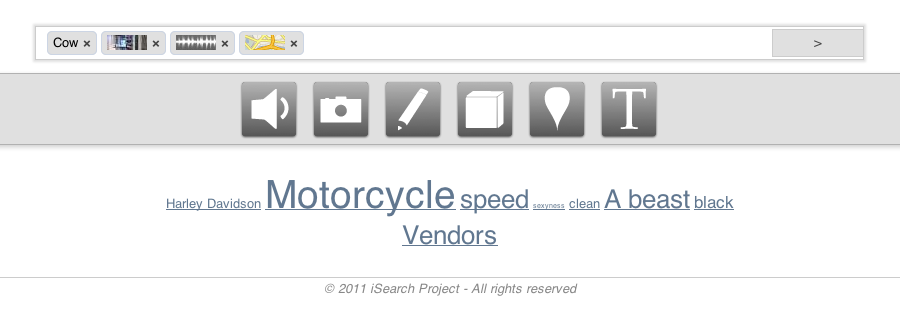
\includegraphics[width=0.8\linewidth]{resources/isearch-UI.png}
  \caption{First version of I-SEARCH interface}
  \label{fig:isearch-ui}
\end{figure}

This interface keeps the idea of a single text box. It is enriched by autocompletion as well as ``tokenization". The term ``Tokenization" refers to the process of representing an item (picture, sound, etc) with a small token in the text field, as if it was part of the text query. We also kept the idea of progressive disclosure for the different actions required by the modes, e.g, upload a picture or sketch something. The different icons are grouped together in a separated menu, close to the main search field.

\subsection{UIIFace}

\subsection{CoFind}

\section{Implementation and Results}
(Jonas, Arnaud)
Talking about the interface itself: 
\begin{itemize}
\item HTML5
\item CSS3 media-queries
\item Compatibility with older browsers
\item Progressive enhancement principle
\end{itemize}

And about the interaction: 
\begin{itemize}
\item Device API
\item audio, video, file API
\item Geolocation and canvas
\item Different sensors used
\item Integration of sensors
\end{itemize}
\section{Evaluation}
(Paul)
Requirement: result criteria
Did you understand the interface
Did you understand the process
2 Use Cases: Rhythm clapping (UC1) and Games (UC7)?

\section{Conclusion and Future Work}
(Tom)

\bibliographystyle{plain}
\bibliography{mmm2012}
\end{document}